\documentclass[oneside]{book}
\usepackage[utf8]{inputenc}
\usepackage{authblk}
\usepackage{setspace} 
\usepackage{amsmath}
\usepackage{textcomp}
\usepackage{amssymb}
\usepackage{geometry}
\usepackage{amsthm}
\usepackage{runic}
\usepackage{mathtools}
\usepackage{graphicx}
\usepackage{mathrsfs}
\usepackage[breaklinks=true,a4paper=true,pagebackref=true]{hyperref}
\graphicspath{ {figures/} }
\geometry{
 a4paper,
 total={170mm,257mm},
 left=20mm,
 top=20mm,
}
\hypersetup{
    colorlinks=true,
    linktoc=true,
    linkcolor=blue,
}
\title{Libraria Calculosis}
\author{Liam Gardner}
\date{\today}
%\doublespacing
\newcommand\tab[1][1cm]{\hspace*{#1}}
\newcommand\nextline{\newline\tab}
\newcommand\nextquestion{\newline\newline}
\newcommand\soln{$\text{sol}^\text{n}\text{ }$}
\newcommand\fs{\mbox{\large $\mathrlap{f}s\,$}\,}
\newcommand\thm[2]{\section*{Theorem: #1}\label{sec:#2}\addcontentsline{toc}{section}{Theorem: #1}}
\newcommand\propn[2]{\section*{Proposition: #1}\label{sec:#2}\addcontentsline{toc}{section}{Proposition: #1}}
\newcommand\ddx[1]{\frac{\text{d}}{\text{dx}}\left[#1\right]}
\newcommand\dydx{\frac{\text{dy}}{\text{dx}}}
\newcommand{\Lim}[1]{\raisebox{0.5ex}{\scalebox{0.8}{$\displaystyle \lim_{#1}\;$}}}
\newcommand{\dfdx}{\frac{\text{df}}{\text{dx}}}
\newcommand \interval[1]{\,^a_b\mathcal{I}_{#1}}
\begin{document}
\DeclarePairedDelimiter\abs{\lvert}{\rvert}

\maketitle
\tableofcontents
\chapter{Approximating $\sqrt{95}$ Using Newton's Method}
\tab
Let $f(x)=x^2-95$, then $f^\prime(x) = 2x$. Newton's Update Function then produces
$$x-\frac{f(x)}{f^\prime(x)}$$
$$=x\frac{x^2-95}{2x}$$
$$=\frac{2x^2}{2x} - \frac{x^2-95}{2x}$$
$$=\frac{x^2+95}{2x}$$
\tab
Thus, we can define a recursive sequence $x_{n+1} = \frac{x_n^2 + 95}{2x_n}$. Using a starting point of $x_0=10$, since $\sqrt{95}$ is close to $\sqrt{100}=10$. we get the following
\nextline
\begin{center}
\begin{tabular}{|c|c|}
\hline
$x_0$ & 10 \\
$x_1$ & 9.75 \\
$x_2$ & 9.764764 \\
\hline
\end{tabular}
\end{center}
\tab
Notice that even for $x_2$, we get an approximation correct to 6 digits.
\subsection{If Newton's method converges, does it always converge to a root?}
\tab
Another way of phrasing this is if $\{x_n\}\rightarrow L$, is $f(L)=0$?.
\nextline
Since the sequence is convergent, we can replace $x_{n+1}$ and $x_n$ with L, and solve $L=L-\frac{f(L)}{f^\prime(L)}$ which implies that $f(L)=0$. Therefore, if Newton's Method converges, we're guaranteed that it converges to a root.	
\chapter{Derivatives of Inverse Functions}
\tab
We still haven't seen $\ddx{\ln(x)}$. Our goal is to relate the derivative of a function with the derivative of its inverse.
Given a function $f(x)$, we can define the linearization at a point $a$ as $\mathcal{L}_a^{f}$. Then, if we invert the linearization function, we get $\left(\mathcal{L}_a^{f}\right)^{-1} = a+\frac{1}{f^\prime(a)}(x-f(a))$. If we take a point $f(a)=b$, then we get that $a= f^{-1}(b)$. Thus $\left(\mathcal{L}_a^f\right)^{-1} = f^{-1}(b) + \frac{x-b}{f^\prime\left(f^{-1}(b)\right)}$. Therefore, we know that the inverse linearization of $f(x)$ at a point $x=a$, is the same as $\mathcal{L}_b^{f^{-1}}$. That is to say, the inverse linearization of a function at a point $a$ is the same as the linearization of the inverse function at a point $f(a)$. Thus, $\mathcal{L}_b^{f^{-1}} = f^{-1}(b) + \ddx{f^{-1}}\lvert_{x=b} \cdot (x-b)$. Thus, by equality we know that $\ddx{f^{-1}}\lvert_{x=b} = \frac{1}{f^\prime(f^{-1}(b))}$
\thm{Inverse Function Theorem}{ift}
\tab
If $f$ is an invertible function on $[c,d]$, differentiable on $(c,d)$, and that $f^\prime(a)\neq0$, then $f^{-1}$ is differentiable at $x=f(a)$ with the derivative $\ddx{f^{-1}}\lvert_{x=b} = \frac{1}{f^\prime(f^{-1}(b))}$. Along with that $\left(\mathcal{L}_a^f\right)^{-1} = \mathcal{L}_{f(a)}^{f^{-1}}$
\subsection{Proof sketch}
\tab
If $f$ is an invertible function, then $f(f^{-1}(x)) = x$. Thus, since they're equal $\ddx{f(f^{-1}(x))} = \ddx{x}$
$$\ddx{f(f^{-1}(x))} = f^\prime(f^{-1}(x))\cdot \ddx{f^{-1}(x)} = 1$$
$$\ddx{f^{-1}(x)} = \frac{1}{f^\prime(f^{-1}(x))}$$
\newline
\null\hfill$\mathcal{QED}$
\subsection{Testing Inverse Function Theorem}
\tab Let $f(x)=x^5$, then $f^{-1}(x)=\sqrt[5]{x}=x^{\frac{1}{5}}$. Thus, we know that $\ddx{f^{-1}(x)} = \frac{1}{5}x^{-4}{5} = \frac{1}{5\cdot\sqrt[5]{x^4}}$.
\nextline
Using IFT, we get that the derivative is $\frac{1}{f^\prime(f^{-1}(x))} = \frac{1}{5(f^{-1}(x))^4}  = \frac{1}{5(x)^\frac{4}{5}}$
\subsection{Derivative of $\ln(x)$}
Using IFT, we can now calculate the derivative of $\ln(x)$.
$$\ddx{\ln(x)} = \frac{1}{f^\prime(f^{-1}(x))} = \frac{1}{e^{\ln(x)}} = \frac{1}{x}$$
\nextline
Furthermore, we can generalize this to know that $\ddx{\log_a(x)} = \frac{1}{x\ln(a)}$
\subsection{Derivative of Inverse Trig Functions}
\tab
We know that $\ddx{\sin(x)} = \cos(x)$. 
$$\ddx{\arcsin{x}}=\frac{1}{\cos(\arcsin(x))}$$
Let $\theta=\arcsin(x)$, then $\sin(\theta)=x$. Using a triangle with a hypotenuse of $1$ and an opposite side to $\theta$ of $x$. Then by the pythagorean theorem, we know the final side $a$ can be found as $a=\sqrt{1-x^2}$. Thus, $\cos(\arcsin(x)) = \cos(\theta) = \sqrt{1-x^2}$
\nextline
Therefore, the derivative of the $\arcsin(x)$ function is $\frac{1}{\sqrt{1-x^2}}$. Similarly, $\ddx{\arccos(x)} = \frac{-1}{\sqrt{1-x^2}}$ and $\ddx{\arctan(x)}=\frac{1}{x^2+1}$.
\chapter{Implicit Differentiation}
\tab
We understand how to take the derivative of explicitly defined functions, as in $y=f(x)$. However, there are ways to differentiate implicitly defined functions, such as $x^2+y^2=1$. That expression implicitly defines two functions. An implicit function is an equation where $y$ is a function of $x$, thus we can (poorly) rewrite the equation for the unit circle as $x^2+f(x)^2 = 1$.
\nextline
To take the derivative of an implicit function, we take the derivative of both sides
$$\ddx{x^2+y^2=1}$$
$$\implies \ddx{x^2+y^2} = \ddx{1}$$
$$\implies \ddx{x^2}+\ddx{y^2} = 0$$
$$\implies 2x + 2y\dydx = 0$$
$$\implies \dydx=\frac{-x}{y}$$
\tab
Often with implicitly defined functions, the result of differentiation will also be implicit.
\nextline
If we wanted to know the slope(s) of the unit circle when $x=\frac{1}{2}$, we can that the two points we get are
$$\left(\frac{1}{2}\right)^2 + y^2 = 1$$
$$\implies y^2 = \frac{3}{4}$$
$$\implies y=\sqrt{\frac{3}{4}}=\frac{\pm\sqrt{3}}{2}$$
\tab
From this, we can use the implicit derivative on both points to get
$$\dydx=\frac{\frac{1}{2}}{\frac{\sqrt{3}}{2}} = \frac{-1}{\sqrt{3}}$$
$$\dydx=\frac{\frac{1}{2}}{\frac{-\sqrt{3}}{2}} = \frac{1}{\sqrt{3}}$$
\tab
Thus, we see that the two slopes of the unit circle at $x=\frac{1}{2}$ are $\frac{\pm1}{\sqrt{3}}$.
\newline
\begin{figure}[h]
\centering
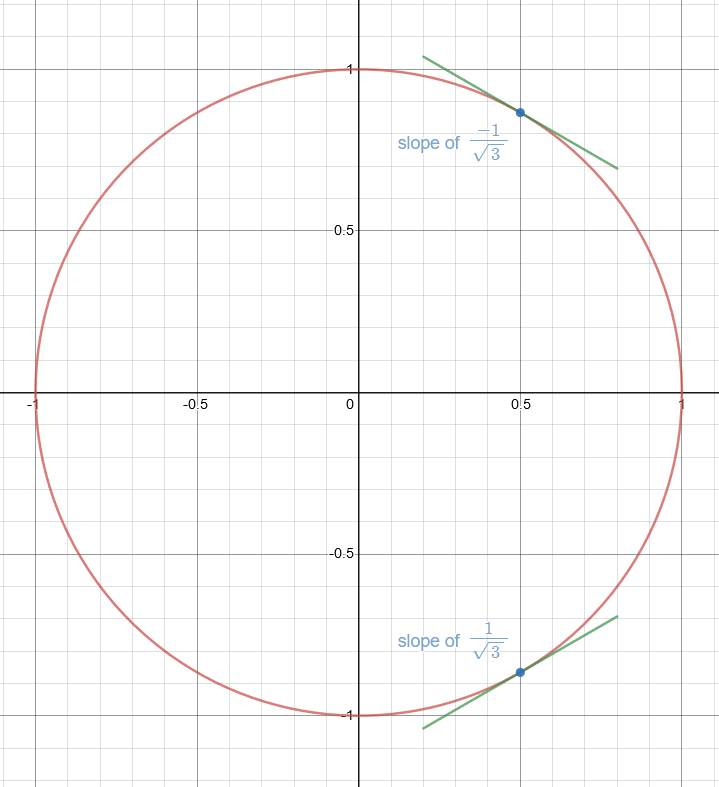
\includegraphics[width=0.35\textwidth]{l24f0}
\caption{Slopes of the unit circle at $x=\frac{1}{2}$}
\end{figure}
\newpage
Trying this again using $x^2+y^2=-1$, we see that the implicit derivative is the same as $x^2+y^2=1$, however, the derivative doesn't actually make sense, as the sum of two squares is always nonnegative. Thus, $x^2+y^2=-1$ does not define a function in $\mathbb{R}^2$, as there are no pairs of real numbers $(x,y)$ that satisfy $x^2+y^2=-1$.
\nextline
Similarly, the relation $2x=x$ defines a point rather than a function, and thus differentiating doesn't yield anything reasonable, as the result is $2=1$. 
\section{Example}
\tab
Find $\dydx$ if $x^3y^5+3x=8y^3+1$
$$\ddx{x^3y^5+3x=8y^3+1}$$
$$\implies \ddx{x^3y^5+3x} = 24y^2\dydx$$
$$\implies \ddx{x^3y^5} + 3 = 24y^2\dydx$$
$$\implies 3x^2y^5 + 5y^4x^3\dydx + 3 = 24y^2\dydx$$
$$\implies \dydx\left(5x^3y^4-24y^2\right)=-3x^2y^5-3$$
$$\implies \dydx=\frac{-3x^2y^5-3}{5x^3y^4-24y^2}$$
\chapter{Logarithmic Differentiation}
\tab
Logarithmic Differentiation is a trick in which you take the natural logarithm of both sides before implicit differentiation.
\nextline
Differentiation with a logarithm gives means of dealing with things like $y=f(x)^{g(x)}$. Along with that, since $\ln(ab)=\ln(a)+\ln(b)$, using logarithmic differentiation allows us to skip using the product rule.
\subsection{Example 1}
Find $\dydx$ for $y=x^x$
\nextline
$$y=x^x$$
$$\implies \ln(y)=\ln(x^x)$$
$$\implies \ln(y)=x\ln(x)$$
$$\implies \ddx{\ln(y)=x\ln(x)}$$
$$\implies \ddx{\ln(y)}=\ddx{x\ln(x)}$$
$$\implies \frac{1}{y}\dydx = \ln(x)+1$$
$$\implies \dydx=y\left(\ln(x)+1\right)$$
\tab
Since the original function was defined explicitly, the derivative should be explicitly defined as well, thus we substitute $y=x^x$ to get
$$\dydx=x^x\left(\ln(x)+1\right)$$
\subsection{Example 2}
Find $\dydx$ for $y=\frac{\sin(x)e^xx^3}{\ln(x)}$
$$y=\frac{sin(x)e^xx^3}{\ln(x)}$$
$$\ln(y)=\ln\left(\frac{\sin(x)e^xx^3}{\ln(x)}\right)$$
$$\implies \ln(y)=\ln(\sin(x))+\ln(e^x)+\ln(x^3)-\ln(\ln(x))$$
$$\implies \ln(y)=\ln(\sin(x))+3\ln(x)-\ln(\ln(x)) + x$$
$$\implies \ddx{\ln(y)=\ln(\sin(x))+3\ln(x)-\ln(\ln(x)) + x}$$
$$\implies \frac{1}{y}\dydx = \frac{\cos(x)}{\sin(x)} + \frac{3}{x} + 1 - \frac{1}{x\ln(x)}$$
$$\implies \dydx=y\left(\frac{\cos(x)}{\sin(x)} + \frac{3}{x} + 1 - \frac{1}{x\ln(x)}\right)$$
\chapter{Extrema}
$\mathbf{\text{def}^{\text{n}}}$: A point $c$ is a local maximum of a function $f$ if there exists an open interval $\mathcal{I}$ containing the point $c$ such that $f(x)\leq f(c) \forall x \in \mathcal{I}$. Similarly, $c$ is a local minimum if $f(x)\geq f(c) \forall x\in\mathcal{I}$. If $f:\mathbb{R}\rightarrow\mathcal{I}$ then $c$ is a global extrema. Thus, all global extrema are also local extrema. It is also true that many local extrema can exist 
\begin{figure}[h]
\centering
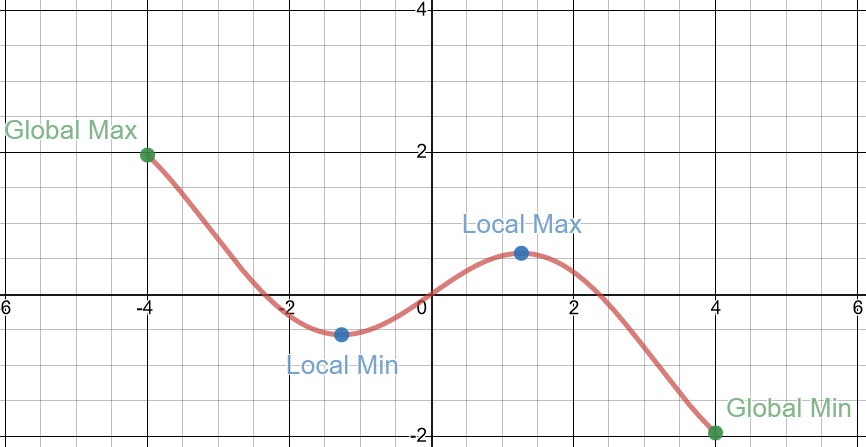
\includegraphics[width=0.5\textwidth]{l25f0}
\caption{Examples of local and global extrema}
\end{figure}

\thm{Local Extrema Theorem}{LET}
\tab
If $c$ is a local extrema and $f^\prime(c)$ exists, then we know $f^\prime(c)=0$.
\subsection{proof}
\tab
Notice that if $c$ is a local min of $f$, we can define a new function $g(x)=-f(x)$ and thus $c$ is a local max of $g$. Now, suppose WLOG suppose $c$ is a local max of $f$. Therefore, there exists an open interval $\mathcal{I}=(a,b)$ containing $c$, such that $f(x)\leq f(c)\forall x\in\mathcal{I}$. Furthermore, suppose that $f^\prime(c)$ exists. Therefore, the following is true:
$$f(c)=\lim_{h\rightarrow0^+}\frac{f(c+h)-f(c)}{h}=\lim_{h\rightarrow0^-}\frac{f(c+h)-f(c)}{h}$$
\tab
If $h>0$ but is small enough that $a<c+h<b$ then we know that $f(c+h)\leq f(c)$ because $c$ is a max of $f$ in the interval $\mathcal{I}$. Therefore, we get that$\frac{f(c+h)-f(x)}{h}\leq 0$ and thus $f^\prime(c)\leq0$
\nextline
If $h<0$ but small ehough that $a<c+h<b$ then we know that $\frac{f(c+h)-f(c)}{h}\geq 0$ since division by a negative flips the inequality sign. Therefore, we get that $f^\prime(c)\geq0$\nextline
Therefore, since $f^\prime(c)\leq0$ and $f^\prime(c)\geq0$ we get that $f^\prime(c)=0$
\newline
\null\hfill$\mathcal{QED}$
\subsection{Converse}
\tab Consider $f(x)=x^3$. Notice now that $f^\prime(x)=3x^2$ and thus $f^\prime(0)=0$, and $f(0)$ isn't a local extrema. Therefore, the converse isn't true. If we also look at $f(x)=\abs{x}$, we know that $f(0)$ is a global min, however the derivative at $x=0$ doesn't exist, and thus the theorem doesn't apply.
\section{Finding Global Extrema}
$\mathbf{\text{def}^{\text{n}}}$: A point $c$ is a critical point of $f^\prime(c)=0$ or $f^\prime(c)$ doesn't exist.\nextline
Let's say that all max/mins occur at critical points. Combining this with the extreme value theorem gives us an algorithm for finding extrema. \nextline
Consider a differentiable function $f$ on the closed interval $[a,b]$. To find all global extrema, we do the following:
\begin{enumerate}
\item find all critical points of $f$ on $[a,b]$, let $\mathcal{C}$ be the set of all $x$-values of critical points.
\item Evaluate $f(a)$, $f(b)$ and $f(c) \forall c\in\mathcal{C}$.
\item Choose the biggest and smallest values of $f(a)$, $f(b)$ and $f(c) \forall c\in\mathcal{C}$ \\
The biggest is the global max, and the smallest is the global min.
\end{enumerate}
\subsection{Example}
Find the max/min of $f(x)=e^{x^3-2x^2-7x}$ on $[0,4]$
\nextline
Finding critical points: We know that $\dfdx$ is defined everywhere, and thus there will be no places on the interval where the derivative is undefined.
\nextline
By the chain rule we know $\dfdx=e^{x^3-2x^2-7x}(3x^2-4x-7)$. Since $e^{p(x)}$ will never be zero, we know that $\dfdx$ will be zero only when the quadratic term is 0. Since the quadratic factors to $(x+1)(3x-7)$, and since we know that $-1\not\in[0,4]$, we know that the only critical point will be $\frac{7}{3}$.
\nextline
$\left\{f(0), f(4), f\left(\frac{7}{3}\right) \right\} = \left\{1, e^4, e^\frac{-392}{27} \right\}$
\nextline
From here, we can see that the global max and min are given by the points $(4,e^4)$, $\left(\frac{7}{3}, e^\frac{-392}{27}\right)$. Therefore, the global max is $4$ and the global min is $\frac{7}{3}$.	
\nextline
This topic will be revisited upon the genesis of the curve sketching unit.
\chapter{The Mean Value Theorem}
\thm{Rolle's Theorem}{RT}
\tab
If $f$ is a continuous function on $[a,b]$ and differentiable on $(a,b)$, and if $0=f(a)=f(b)$, then $\exists c\in (a,b)$ such that $f^\prime(c)=0$.
\subsection{Proof}
\tab
Suppose that $f$ is continuous on $[a,b]$ and differentiable on $(a,b)$ with $f(a)=f(b)=0$.
\subsection*{Case 1}
\tab $\exists x_0\in(a_b)$ with $f(x_0)>0$. The Extreme Value Theorem, shows that $f(x)$ achieves a max value on $[a,b]$. We know that the maximum point $c\in (a,b)$  is thus not at the endpoints. Hence, since $f^\prime(c)$ exists, by the \hyperref[sec:LET]{Local Extrema Theorem} we know that $f^\prime(c)=0$.
\subsection*{Case 2}
\tab $\exists x_0\in(a,b)$ with $f(x_0)<0$. The Extreme Value Theorem shows that $f(x)$ achieves a min value on $[a,b]$. We know that the minimum point $c\in(a,b)$ is thus not at the endpoints. Hence, since $f^\prime(c)$ exists, by the \hyperref[sec:LET]{Local Extrema Theorem} we know that $f^\prime(c)=0$.
\subsection*{Case 3}
\tab $f:[a,b]\rightarrow 0$, hence $f^\prime:(a,b)\rightarrow 0$ and thus there are lots of choices for $c$.
\thm{The Mean Value Theorem}{MVT}
\tab
Suppose $f$ is continuous on $[a,b]$ and differentiable on $(a,b)$. Then, $\exists c\in(a,b)$ such that $f^\prime(c)=\frac{f(b)-f(a)}{b-a}$. Rolle's Theorem is a special case of Mean Value Theorem.
\subsection{Proof}
\tab Let $h(x)=f(x)-f(a)-\left(\frac{f(b)-f(a)}{b-a}\right)(x-a)$. Notice that $h(a)=h(b)=0$. Since $h$ is continuous on $[a,b]$ and differentiable on $(a,b)$. Thus, since the conditions of Rolle's Theorem are met, we know that $\exists c\in(a,b)$ such that $h^\prime(c)=0$.\nextline
$$\ddx{h^\prime(x)}\lvert_{x=c}=f^\prime(c)-\frac{f(b)-f(a)}{b-a}=0$$
\tab
Therefore, we get that $f^\prime(c)=\frac{f(b)-f(a)}{b-a}$.
\subsection{Examples}
\tab\textit{Find all points $c$ that satisfy the mean value theorem for} $f(x)=x^3+2x^2-x$ on $[-1,2]$\nextline
By MVT we know that $f^\prime(c)=\frac{f(2)-f(-1)}{2-(-1)} = \frac{14-2}{3} = 4$. Therefore, there is a point $c$ where the derivative is equal to 4. $f^\prime(x)=3x^2+4x-1$
$$f^\prime(x)=3x^2+4x-1=c$$
$$x=\frac{-4\pm\sqrt{76}}{6}$$
\tab Since $\frac{-4-\sqrt{76}}{6}\not\in [-1,2]$, we know that it is not a proper value of $c$. Therefore, the only value of $c$ for this interval is $c=\frac{\sqrt{76}-4}{6}$
\newline
\nextline
\textit{Suppose that a function $f$ is continuous and differentiable everywhere. Furthermore, suppose $f$ has two roots. Then show $f^\prime$ has at least one root}
\nextline
Let $a,b$ be distinct roots of $f$, then $f(a)=f(b)=0$. Thus, by Rolle's Theorem, we know that $\exists c\in(a,b)$ such that $f^\prime(c)=\frac{f(b)-f(a)}{b-a}=0$ and thus there is at least one root of $f^\prime$.
\section{Applications of MVT}
\tab
$\text{Def}^{\text{n}}$: A function $F$ is called an antiderivative of $f$ is $F^\prime(x)=f(x) \forall x\in\mathbb{R}$
\nextline
$F(x)=\frac{x^2}{2}$ is an antiderivative of $f(x)$, since $F^\prime(x)=\frac{2x}{2}=x=f(x)$

\thm{The Constant Function Theorem}{CFT}
\tab
If $f^\prime(x)=0$ $\forall x\in\mathcal{I}$ then $f(x)=c$ $\forall x\in\mathcal{I}$.
\subsection{Proof}
\tab
Let $\mathcal{I}$ be some interval, then suppose $f^\prime(x)=0$ $\forall x\in\mathcal{I}$. Note that $f$ is continuous on $\mathcal{I}$. Let $x_1, x_2\in \mathcal{I}$ where $x_1\neq x_2$. Then, let $f(x_1)=k$. By the Mean Value Theorem, $\exists c\in(x_1,x_2)$ such that $f^\prime(c)=\frac{f(x_2)-f(x_1)}{x_2-x_1}$. Since $(x_1,x_2)\subseteq \mathcal{I}$, we know that $f^\prime(c)=0$ and thus $\frac{f(x_2)-f(x_1)}{x_2-x_1}=0\implies f(x_2)-f(x_1)=0\implies f(x_2)=f(x_1)=k$.
\nextline
Since both $x_1$ and $x_2$ were arbitrary, we conclude that $f(x)=k$ $\forall x\in\mathcal{I}$
\thm{Uniqueness of Antiderivatives}{UA}
\tab
Antiderivatives are not unique, since if we take $F(x)=h(x)+c$ and $f(x)=h^\prime(x)$ then $F^\prime(x)=h^\prime(x)=f(x) \forall c\in\mathbb{R}$. However, outside of adding constants, antiderivatives are unique (although it is not straightforward). This can be shown using the Mean Value Theorem.
\nextline
If $f^\prime(x)=g^\prime(x)$ $\forall x\in\mathcal{I}$, and thus $f(x)$ and $g(x)$ are antiderivatives of the same function, then $\exists k\in\mathbb{R}$ such that $f(x)=g(x)+k$ $\forall x\in\mathcal{I}$.
\subsection{Proof}
Let $h(x)=f(x)-g(x)$ and thus $h^\prime(x)=f^\prime(x)-g^\prime(x)=0$ $\forall x\in\mathcal{I}$. Hence, by \hyperref[sec:CFT]{The Constant Function Theorem}, $\exists k\in\mathbb{R}$ such that $h(x)=k$ $\forall x\in\mathcal{I}$. Therefore, $h(x)=f(x)-g(x)=k$ $\forall k\in\mathcal{I}\implies f(x)=g(x)+k$ $\forall x\in\mathcal{I}$.
\subsection{Notation}
The family of antiderivatives for a function $f(x)$ is denoted as follows, where $f(x)$ is referred to as the ``integrand'' and the dx is referred to as the ``variable of integration''.
$$F(x)=\int f(x)\text{ dx}$$
\tab As an example, $\int x^2\text{ dx} = \frac{x^2}{2}$
\thm{Increasing/Decreasing Function Theorem}{IncFT}
\tab
Let $\mathcal{I}$ be some interval with $x_1,x_2\in\mathcal{I}$ where $x_1< x_2$.
\begin{enumerate}
\item If $f^\prime(x)>0 \,\forall x\in\mathcal{I}$ then, $f(x_2)>f(x_1)$ and we say $f$ is \textit{increasing} on $\mathcal{I}$
\item If $f^\prime(x)\geq0 \,\forall x\in\mathcal{I}$ then, $f(x_2)\geq f(x_1)$ and we say $f$ is \textit{non-decreasing} on $\mathcal{I}$
\item If $f^\prime(x)<0 \,\forall x\in\mathcal{I}$ then, $f(x_2)<f(x_1)$ then we say $f$ is \textit{decreasing} on $\mathcal{I}$
\item If $f^\prime(x)\leq0 \,\forall x\in\mathcal{I}$ then, $f(x_2)\leq f(x_1)$ and we say $f$ is \textit{non-increasing} on $\mathcal{I}$
\end{enumerate}
\subsection{Proof of (1)}
\tab
Let $\mathcal{I}$ be an interval such that $x_1<x_2 \in\mathcal{I}$. Suppose that $f^\prime(x)>0\,\forall x\in\mathcal{I}$. Since $f^\prime$ exists, we know that $f$ is continuous $\forall x\in\mathcal{I}$. We can thus apply \hyperref[sec:MVT]{The Mean Value Theorem} to $[x_1, x_2]$.\nextline
$\exists c\in(x_1,x_2)$ such that $\frac{f(x_2)-f(x_1)}{x_2-x_1} = f^\prime(c)$. Since we know $f^\prime(c)>0$ and $x_2-x_1>0$, we know that $f(x_2)-f(x_1)>0$. Thus, $f$ is increasing over $\mathcal{I}$.
\subsection{Converses}
\tab
The converse of (2) and (4) are true (if $f(x)$ is non-increasing/non-decreasing on $\mathcal{I}$ then $f^\prime(x) >0 \,\forall x\in\mathcal{I}$).
\nextline
The converse of (1) and (3) are false. Consider $f(x)=x^3$. Where $f(x_2)>f(x_1) \forall x_2>x_1$ However, $f^\prime(0)=0$.
\section{Functions with Bounded Derivatives}
What information can we derive from a function $f$ if we know the bounds of $\dfdx$?
\nextline
Suppose $m\leq \dfdx \leq M$ $\forall x\in(a,b)$. If $f$ is continuous on $[a,b]$ then we can use \hyperref[sec:MVT]{Mean Value Theorem}.
\nextline
Let $x\in(a,b)$. Applying MVT we get $\exists c\in(a,x)$ with $f^\prime(c) = \frac{f(x)-f(a)}{x-a}$.
$$m \leq f^\prime(c) =\frac{f(x)-f(a)}{x-a} \leq M$$
$$m(x-a) \leq f(x)-f(a) \leq M(x-a)$$
$$f(a) + m(x-a) \leq f(x) \leq f(a) + M(x-a)$$
\tab
This implies that $f(x)$ is bounded between two lines.
\thm{Bounded Derivative Theorem}{BDT}
\tab
If a function $f$ is continuous on $\interval{o}$ and differentiable on $\interval{c}$ with $m\leq f^\prime(x)\leq M$ $\forall x\in\interval{o}$ then $f(a)+m(x-a)\leq f(x)\leq f(a)+M(x-a)$ $\forall x \in\interval{c}$.
\subsection{Example}
Show that $\ln(3)\in\left[\frac{7-e}{4}, \frac{3}{e}\right]$\nextline
Let $f(x)=\ln(x)$. Hence, $f^\prime(x)=\frac{1}{x}$. We need to bound $f^\prime(x)$ to use the theorem. Thus, we need some interval $\interval{c}$ with $a<3<b$. We also need $f(a)$ to be easily computable. If we take $a=e$ then $\ln(a)=1$. and $1<3$. Since we don't need $f(b)$ to be easily computable, we can take $b=4$.
\nextline
Note that $\ddx{\frac{1}{x}} = \frac{-1}{x^2}$. Thus, from the \hyperref[sec:IncFT]{Increasing Function Theorem} we know that $f^\prime(x)$ is decreasing. Thus, $f^\prime(4) \leq f^\prime(x) \leq f^\prime(e)$. Since the derivative can be bound between $\frac{1}{4}$ and $\frac{1}{e}$, the natural choice for a range would be $f^\prime(x)\in\left[\frac{1}{4}, \frac{1}{e}\right]$.
\nextline
$$f(a) + m(x-a) \leq f(x) \leq f(a)+M(x-a)$$
$$1 + \frac{1}{4}(x-e) \leq f(x) \leq f(a)+\frac{1}{e}(x-a)$$
$$1 + \frac{1}{4}(3-e) \leq f(x) \leq 1 + \frac{1}{e}(x-e)$$
$$\frac{7-e}{4} \leq f(x) \leq \frac{3}{e}$$
\newline
\null\hfill$\mathcal{QED}$
\nextline
Check out the example in the textbook that uses Bounded Derivative Theorem to show the following;
$$\lim_{n\rightarrow\infty} \left(1+\frac{1}{n}\right)^n = e$$
\section{Comparing Functions Using Derivatives}
Suppose $f$ and $g$ are continuous at $x=a$ and $f(a)=g(a)$
\begin{enumerate}
\item If $f^\prime(x) < g^\prime(x)$ $\forall x>a$ then $f(x)<g(x)$ $\forall x>a$
\item If $f^\prime(x) > g^\prime(x)$ $\forall x>a$ then $f(x)>g(x)$ $\forall x>a$
\item If $f^\prime(x) \leq g^\prime(x)$ $\forall x>a$ then $f(x)\leq g(x)$ $\forall x>a$
\item If $f^\prime(x) \geq g^\prime(x)$ $\forall x>a$ then $f(x)\geq g(x)$ $\forall x>a$
\end{enumerate}
\subsection{Proof of (3)}
\tab
Suppose $f$ and $g$ are continuous at $x=a$ with $f(a)=g(a)$ and $f^\prime(x) \leq g^\prime(x)$ $\forall x>a$.
\nextline
Let $h(x)=f(x)-g(x)$. Then $h(a)=f(a)-g(a)=0$. Let $x>a$, $h^\prime(x)=f^\prime(x)-g^\prime(x)$. By the hypothesis, we know that when $x>a$ that $f^\prime(x)\leq g^\prime(x)$, thus, by the \hyperref[sec:IncFT]{Decreasing Function Theorem}. Hence, $h(x)\leq 0\implies f(x)-g(x)\leq 0\implies f(x)\leq g(x)$ $\forall x>a$.
\end{document}